\documentclass[10pt,a4paper]{article}
\usepackage[margin=18mm]{geometry}
\usepackage[T1]{fontenc}
\usepackage{pdflscape}
\usepackage{lmodern,microtype,amsmath,amssymb,booktabs,tabularx,longtable,array,float,caption,xcolor,enumitem,siunitx,tikz}
\usetikzlibrary{arrows.meta,positioning,calc}
\usepackage[colorlinks=true,urlcolor=blue!55!black,citecolor=blue!55!black,linkcolor=blue!55!black]{hyperref}
\usepackage[backend=biber,style=ieee,sorting=none,doi=true,url=false]{biblatex}
\addbibresource{boat_references.bib}
\definecolor{navy}{RGB}{26,57,81}\definecolor{teal}{RGB}{18,118,132}\definecolor{cream}{RGB}{245,250,251}
\setlength{\parindent}{0pt}\setlength{\parskip}{5pt}\renewcommand{\arraystretch}{1.24}\setlength{\tabcolsep}{4.0pt}
\newcolumntype{Y}{>{\raggedright\arraybackslash}X}
\newcolumntype{L}[1]{>{\raggedright\arraybackslash}p{#1}}
\title{\color{navy}\bfseries Portable Microplastic Survey Boat -- V2.3\\[3pt]\large Critical Component Procurement, Comparisons, Payload and Mission Feasibility}
\author{Year 3 Engineering Group Project --- preliminary systems design}\date{2 November 2026 --- Version 2.3}
\begin{document}\maketitle
\tableofcontents
\begin{abstract}This Version 2.3 report retains the Version 1 engineering calculations and adds university-approved supplier listings, traceable MYR prices, detailed published electrical/mechanical specifications, and datasheet/quotation gaps. All motor and motorised-pump purchase candidates in this revision are sold by an approved supplier. It translates the requirement to produce a spatial microplastic concentration heat map across a $20\,\mathrm{m}\times20\,\mathrm{m}$ water area within about two hours into a first-pass hull, propulsion, autonomy, pump, communications, and energy architecture. Manufacturer-rated values are cited separately from illustrative engineering assumptions. It does \emph{not} establish waterproof marine-motor qualification, actual propulsive thrust, boat top speed, sensor selectivity or two-hour field performance. The companion methodology review contains the scientific measurement screening.\end{abstract}

\section{Version 2 procurement scope and evidence rules}
\textbf{Procurement rule.} The approved/registered supplier list was provided by the project team. A website listing is \emph{not} itself proof of the university's purchase-order status: the department must confirm the current account, delivery and quote requirements. Registered suppliers have no minimum purchase value according to the provided purchase instructions. Non-registered buying is a fallback \emph{only} when a registered supplier cannot fulfil the item, and requires prior Procurement Department coordination with \href{mailto:Radha.Sivadasan@nottingham.edu.my}{Radha.Sivadasan@nottingham.edu.my}.

\textbf{Price evidence dated 2 November 2026.} All amounts in the comparison tables are \textbf{listed MYR prices observed on approved Malaysian seller webpages or expressly allowed Shopee marketplace listings}, not a binding quotation. They may change, and tax, delivery, quantity tiers and compatibility accessories are not included unless a listing explicitly says otherwise. Each compared product has a directly clickable \textcolor{teal}{\textbf{listing}} link, and each item needing a supplier reply is marked \textbf{RFQ} (request for quotation). \textbf{Shopee prices are separately labelled as public marketplace listings and are not substituted for a registered-supplier quotation.}

\begin{table}[H]\centering\footnotesize
\caption{Selected approved electronics suppliers and website access. Supplier names and restrictions come from the university project purchase instructions.}
\begin{tabularx}{\linewidth}{@{}L{3cm}Y L{3.1cm}@{}}\toprule
Supplier & Verified Malaysian storefront / contact & V2 role \\\midrule
Cytron & \href{https://my.cytron.io/}{my.cytron.io} & Itemised public prices \\
GI Electronic & \href{https://www.gie.com.my/}{gie.com.my} & Camera price comparison \\
Element14 & \href{https://my.element14.com/}{my.element14.com} & RFQ / alternates \\
RS & \href{https://my.rs-online.com/web/}{my.rs-online.com} & RFQ / protected electricals \\
DigiKey & \href{https://www.digikey.my/en}{digikey.my} & RFQ / traceable parts \\
Autobotic, Mybotic & University-listed vendors; website/product listing not verified here & Direct RFQ \\
Vanguard KL & \href{mailto:enquiry@vanguardelectronic.com.my}{Email procurement enquiry} & Direct RFQ \\
\bottomrule\end{tabularx}\end{table}
\textbf{Other registered procurement routes:} for hull manufacture and waterproof fittings, approach YLT Hardware (\href{mailto:atikah_ylthardware@outlook.com}{email}), Grandtech Engineering (\href{mailto:adnan_matsarip@yahoo.com.my}{email}), Multi Impact (\href{mailto:Yang@multiimpact.com.my}{email}) and LCG Scientific (\href{mailto:lcgscientificl@gmail.com}{email}). The provided list restricts Dynamics Industrial (\href{mailto:dynamicinds@gmail.com}{email}) to \emph{electrical only}. JL Brilliant Resources (\href{mailto:jlbresources2133@gmail.com}{email}) and TX Moon (\href{mailto:ray.txmoon@gmail.com}{email}) are the registered \emph{online-items} routes. Their product-specific prices are \textbf{RFQ}, not zero.

\section{Mission requirements, operating modes and acceptance criteria}
A $400\,\mathrm{m}^2$ water survey must yield georeferenced observations and a rendered 2D concentration or explicitly provisional particle proxy map inside 120 minutes. Track A measures aboard a moving or stopped boat; Track B collects known-volume labelled water at 16 illustrative grid locations for portable shoreline analysis. Remote operator retains positive control and a safe manual retrieval plan. The shoreline/boat route, local current, obstacle map, GNSS performance, wind and water depth are not specified and require field reconnaissance.

\begin{table}[H]\centering\footnotesize
\caption{Proposed acceptance gates; numerical criteria are design targets, not published hardware performance.}
\begin{tabularx}{\linewidth}{@{}L{3.1cm}Y Y@{}}\toprule
Dimension & Acceptance demonstration & Consequence if failed\\\midrule
Geospatial output & $20\times20$ m map, original locations, timestamps, size limits, data-quality legend & Map fails stakeholder purpose\\
Timeliness & First deployment to completed map within $\leq120$ min & Reduce stations or improve throughput\\
Measurement credibility & Controlled known-particle trials, river interferents, measured sample volume, blanks & Label ``suspected MP-like particles'' or calibrated proxy\\
Navigation & Confirm track spacing and positional error; manual RC override & No autonomous close-range operation\\
Flotation & Float full wet load with reserve buoyancy and stable freeboard & Increase hull displaced volume\\
Energy & 120 min at \emph{measured} average load, BMS/fuse adequate for transients & More battery, lower draw or mission redesign\\\bottomrule\end{tabularx}\end{table}

\section{Architecture and critical component list}
\begin{figure}[H]\centering
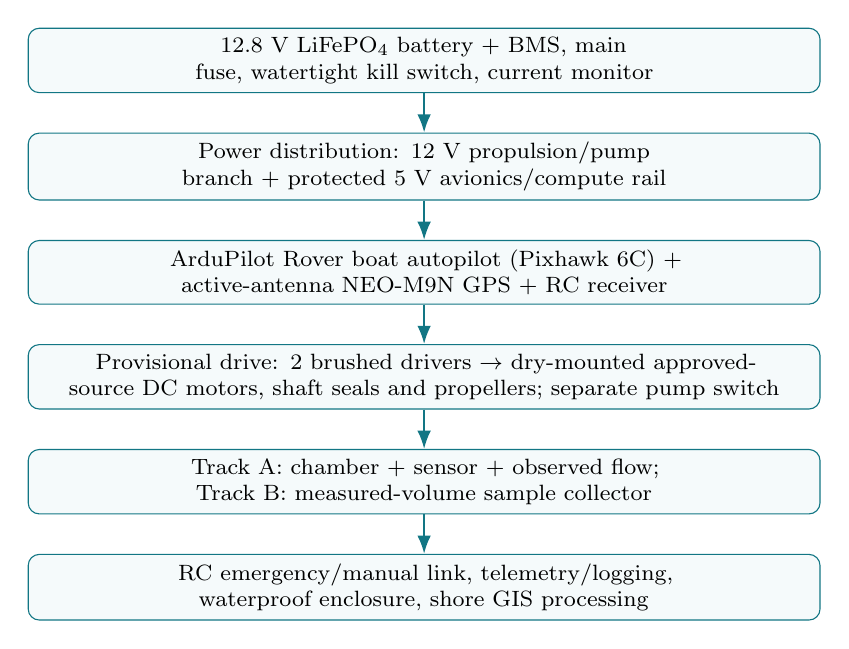
\begin{tikzpicture}[>=Latex,node distance=5mm,b/.style={draw=teal,rounded corners,fill=cream,align=center,text width=0.81\linewidth,minimum height=8mm,font=\footnotesize},a/.style={-Latex,thick,teal}]
\node[b] (bat){12.8 V LiFePO$_4$ battery + BMS, main fuse, watertight kill switch, current monitor};
\node[b,below=of bat] (pdb){Power distribution: 12 V propulsion/pump branch + protected 5 V avionics/compute rail};
\node[b,below=of pdb] (control){ArduPilot Rover boat autopilot (Pixhawk 6C) + active-antenna NEO-M9N GPS + RC receiver};
\node[b,below=of control] (drivers){Provisional drive: 2 brushed drivers $\rightarrow$ dry-mounted approved-source DC motors, shaft seals and propellers; separate pump switch};
\node[b,below=of drivers] (sample){Track A: chamber + sensor + observed flow; Track B: measured-volume sample collector};
\node[b,below=of sample] (link){RC emergency/manual link, telemetry/logging, waterproof enclosure, shore GIS processing};
\foreach \u/\v in {bat/pdb,pdb/control,control/drivers,drivers/sample,sample/link} \draw[a] (\u)--(\v);
\end{tikzpicture}
\caption{Block diagram (logical, not complete wiring schematic). RC safety and boat-side logs must not depend on the data-telemetry link.}\end{figure}
\begin{table}[H]\centering\scriptsize
\caption{Prototype system purchase priorities; masses are budget allowances unless specified by manufacturers.}
\begin{tabularx}{\linewidth}{@{}L{2.3cm}L{3.1cm}Y@{}}\toprule
Critical system & Candidate hardware & Procurement/check before commitment\\\midrule
Hull/buoyancy & 2 sealed cylindrical pontoons, $0.90$ m long $\times0.20$ m OD, rigid platform & Measure true sealed displacement, frame strength and wet load\\
Propulsion & 2 registered-supplier 12 V geared DC motors + sealed shafts/propellers, or 2 Shopee brushless marine propulsors + matching ESCs & \textbf{Bench-only until water testing}; marine Shopee offerings not yet engineering-qualified\\
Autopilot & Holybro Pixhawk 6C, ArduPilot Rover firmware & Supported hardware; boat mode uses \texttt{FRAME\_CLASS=2} \cite{Pixhawk6C,ArduBoat}\\
RC link & RadioMaster Pocket 2.4 GHz ELRS with matched serial receiver & Manually test kill/hold/failsafe; ensure regional radio compliance \cite{RadioMaster}\\
Telemetry & 2.4 GHz Wi-Fi for near-bank test; optional compatible SiK pair & MAVLink/logs and onboard SD backup, independent of RC \cite{SiK}\\
GNSS & u-blox \textbf{NEO-M9N-00B} module + compatible powered active L1 antenna/compass unit & Verify receiver board has antenna bias circuitry, magnetometer and correct autopilot cable \cite{M9N,SparkM9N}\\
Sampling & Cytron R385 12 V diaphragm pump + calibrated flowmeter & Nominal 1.6 L/min needs an in-line filter-load test before use\\
Power & 12.8 V 20 Ah LiFePO$_4$, integrated BMS, LiFePO$_4$ charger & Peak current and fuse coordination; avoid powering motor from flight-controller rail \cite{Bioenno,PM02D}\\
Safety & Sealed electronics, buoyant tether/recovery aid, prop guards, water-leak detector & Safety switch, loss-of-RC configuration, emergency hand retrieval\\\bottomrule\end{tabularx}\end{table}


\begin{landscape}
\section{Engineering specification comparison dossier (V2.3)}
\textbf{Scope and definitions.} These expanded tables cover the priced approved-supplier candidates from V2 and reference-only non-motor electronic hardware. Every compared propulsion motor is sold either by an approved registered vendor or on Shopee Malaysia. Pump motors and motor drivers have registered-vendor listings. \textbf{NR} means a field is not published in the identified source, not zero. \textbf{RFQ} means no approved-supplier product-specific price has been substantiated. A \emph{supplier} link denotes an approved seller; a \emph{spec} link denotes manufacturer documentation, a supplier's technical product page, or an explicit equipment reference. Links labelled \emph{spec} are not all downloadable PDF datasheets. Pricing in RM is an indicative 2 November 2026 listing, not a quote. \textbf{Do not compare unlike outputs}: water-jet static thrust (kgf), brushed motor output shaft torque (N m), pump flow (L/min) and sensor response have different meanings.

\subsection{Approved-supplier motor comparison: detailed electrical and mechanical specifications}
\textbf{Strict purchasing constraint.} The first table compares dry-shaft gearmotors available from registered suppliers (Cytron or GI Electronic). The following table gives dedicated submersible thrusters sold on Shopee Malaysia, the additional marketplace expressly allowed by the project team. Shopee listings do not by themselves establish registered-supplier procurement approval. \textbf{None of these listed gearmotors is documented as a waterproof marine thruster.} They are candidates for a dry-mounted shaft-drive proof of concept after the group designs and validates shaft seals, propeller coupling, mounts and guards. For a true ready-made underwater thruster, submit the same specification checklist as an RFQ through one of the listed approved electronics suppliers; do not assume any brand is supplied by them without written confirmation.

\textbf{Output and efficiency definitions:} $P_{\rm shaft}=\tau(2\pi n/60)$ is a derived shaft-output \emph{estimate} at the supplier's stated rated torque and loaded RPM; $P_{\rm elec}=VI_{\rm rated}$ is electrical input \emph{at that same stated point}. Mechanical horsepower = $P_{\rm shaft}/745.7$; this is \emph{not} motor nameplate HP, thrust, boat speed, or battery load at stall. In a true datasheet, verify that torque and speed are jointly specified. Calculated values below carry the label C. 'NR' means the exact value is not reported by the linked listing (not 0).

\scriptsize\setlength{\tabcolsep}{2.7pt}\renewcommand{\arraystretch}{1.42}
\begin{longtable}{@{}L{27mm}L{17mm}L{20mm}L{13mm}L{29mm}L{30mm}L{30mm}L{24mm}L{14mm}L{26mm}@{}}
\caption{\textbf{Approved-supplier propulsion gearmotors only}: supplier-derived specs and explicitly calculated shaft output. Dimensions are the motor/gearbox envelope unless stated otherwise.}\label{tab:approvedmotors}\\
\toprule
\textbf{Model / vendor} & \textbf{Supply, style} & \textbf{Dimensions / shaft} & \textbf{Weight} & \textbf{Rated torque and loaded speed} & \textbf{Output shaft W / hp (C)} & \textbf{Rated I / stall I} & \textbf{Input W rated / max} & \textbf{RM /pc} & \textbf{Product / datasheet}\\\midrule\endfirsthead
\multicolumn{10}{l}{\textit{Approved-supplier motor comparison (continued)}}\\\toprule
\textbf{Model / vendor} & \textbf{Supply, style} & \textbf{Dimensions / shaft} & \textbf{Weight} & \textbf{Rated torque and loaded speed} & \textbf{Output shaft W / hp (C)} & \textbf{Rated I / stall I} & \textbf{Input W rated / max} & \textbf{RM /pc} & \textbf{Product / datasheet}\\\midrule\endhead\bottomrule\endfoot
\textbf{Cytron GM25 20K} & 12 V brushed, 20:1 & 25-mm family; full length NR & NR & 0.225 N m at 780 rpm & \textbf{18.38 W / 0.02465 hp} (C) & 2.7 A / $<16$ A & 32.4 W / $<192$ W (C, stall upper bound) & \textbf{49.00} & \href{https://my.cytron.io/c-dc-geared-motor/p-12v-980rpm-2.3kgfcm-high-power-brushed-dc-geared-motor}{supplier + spec}; formal PDF NR\\
\textbf{Cytron GM25 34K} & 12 V brushed, 34:1 & 21.5-mm gearbox length; full envelope NR & NR & 0.340 N m at 560 rpm & \textbf{19.94 W / 0.02674 hp} (C) & 2.7 A / $<16$ A & 32.4 W / $<192$ W (C, stall upper bound) & \textbf{49.00} & \href{https://my.cytron.io/c-dc-motor/p-12v-580rpm-3.5kgfcm-high-power-brushed-dc-geared-motor}{supplier + spec}; formal PDF NR\\
\textbf{Cytron SPG30 GR30} & 12 V brushed, 30:1 & 37-mm motor diameter; shaft 6 x 15 mm; full length NR & NR & 1.14 kgf cm (0.1118 N m), 266 rpm & \textbf{3.11 W / 0.00418 hp} (C) & 0.40 A / 1.2 A stall & 4.8 W / 14.4 W stall (C) & \textbf{49.00} & \href{https://my.cytron.io/p-12v-37mm-dc-geared-motor}{supplier}; \href{https://drive.google.com/drive/folders/1DSM3_qSWDYrgrl4ePLlrXPHIkHGKmAHj}{datasheet folder}\\
\textbf{Cytron SPG30 GR56} & 12 V brushed, 56:1 & 37-mm motor diameter; shaft 6 x 15 mm; full length NR & NR & 2.1 kgf cm (0.2060 N m), 112 rpm & \textbf{2.42 W / 0.00324 hp} (C) & 0.40 A / 1.2 A stall & 4.8 W / 14.4 W stall (C) & \textbf{49.00} & \href{https://my.cytron.io/p-12v-37mm-dc-geared-motor}{supplier}; \href{https://drive.google.com/drive/folders/1DSM3_qSWDYrgrl4ePLlrXPHIkHGKmAHj}{datasheet folder}\\
\textbf{GI E0180018 15 W} & 12 V brushed, 100:1 & Diameter / total length NR; 6-mm D-shaft & 310 g & 10 kgf cm (0.9807 N m), 45 rpm & \textbf{4.62 W / 0.00620 hp} (C) & 0.95 A / stall NR & 11.4 W (C); maker class ``15 W''; max NR & \textbf{52.10} & \href{https://www.gie.com.my/shop.php?action=robotics/motors/gearmotor_555}{supplier + technical spec}; PDF NR\\
\end{longtable}
\end{landscape}


\begin{landscape}
\subsection{Waterproof thruster alternatives on Shopee Malaysia -- procurement-permitted, not yet engineering-qualified}
\footnotesize\setlength{\tabcolsep}{3pt}\renewcommand{\arraystretch}{1.46}
\begin{longtable}{@{}L{31mm}L{25mm}L{27mm}L{22mm}L{30mm}L{31mm}L{28mm}L{16mm}L{35mm}@{}}
\caption{\textbf{Shopee Malaysia underwater propulsion motor listings}: only product-specific Shopee offers are used for MYR purchase prices. ``Reference'' figures from model-identical listings outside the approved purchase channels are technical leads, \emph{not verified specs for the Shopee variant}.}\label{tab:shopeemarine}\\
\toprule
\textbf{Motor / source} & \textbf{Voltage and technology} & \textbf{Dimensions} & \textbf{Mass} & \textbf{Mechanical output, thrust, horsepower} & \textbf{Loaded draw / input power} & \textbf{Max current and other limits} & \textbf{RM/pc} & \textbf{Shopee price / spec source}\\\midrule\endfirsthead
\multicolumn{9}{l}{\emph{Shopee marine motor comparison continued}}\\\toprule
\textbf{Motor / source} & \textbf{Voltage and technology} & \textbf{Dimensions} & \textbf{Mass} & \textbf{Mechanical output, thrust, horsepower} & \textbf{Loaded draw / input power} & \textbf{Max current and other limits} & \textbf{RM/pc} & \textbf{Shopee price / spec source}\\\midrule\endhead\bottomrule\endfoot
\textbf{4-blade thruster, Weihua.my} (Shopee) & 12--24 V, DC (motor type / ESC inclusion NR) & NR; request dimensioned drawing & NR & Static thrust, torque, shaft W and hp all NR; seller provides no thrust curve & NR; \textbf{13 A in title} is unverified operating condition; 12--24 V $\times$ 13 A = 156--312 W \emph{only as a voltage-current product}, not rated power & Peak, thermal and continuous duty NR; 5 purchase variations & \textbf{94.96} (after voucher; variant uncertain) & \href{https://shopee.com.my/12V-24V-13A-Underwater-Thruster-Motor-4-Blades-Propeller-for-ROV-RC-Bait-Boat-i.925574334.25165471266}{Shopee listing}; formal datasheet NR \\
\textbf{M060 deepwater brushless, Shuaichi Hobby} (Shopee) & 12--24 V BLDC in listing; 24 V rated on comparable \emph{unmatched} vendor description & Comparable M060 \emph{reference} 90 mm long $\times$ 69 mm fairing diameter; exact Shopee variant NR & Reference ~200 g dry; actual listed variant NR & Shopee actual thrust curve / shaft W / hp NR; generic M060 model reference claims forward 3.46 kgf at 24 V, \emph{unverified for this listing} & Reference rated input 140 W at 24 V; current 6 A claimed; bench point for Shopee variation NR & Reference 6 A max, but exact Shopee variant, sealing pressure and ESC rating must be confirmed; ``200 m'' is a vendor claim & \textbf{282.32} (after voucher) & \href{https://shopee.com.my/M060-200m-Deepwater-Thruster-Waterproof-Brushless-DC-Motor-ROV-Propulsor-12V-24V-Parts-for-RC-Unmanned-Ship-Underwater-Robot-i.133237764.45758558847}{Shopee listing}; \href{https://www.coupang.com/vp/products/9065031801}{comparative model description, not a datasheet} \\
\textbf{FSM3660 360KV, ihhh\_5654} (Shopee) & 12--24 V BLDC, 360 KV seller title & Exact assembly dimensions NR; model ``3660'' does \emph{not} confirm complete propeller housing envelope & ~260 g from matched-model \emph{reference}; exact SKU mass NR & Thrust/shaft output and horsepower NR; 360 KV is rpm per volt no-load gradient, \emph{not} rated rpm under load & Matched-model reference gives 6.5--11.6 A continuous, \emph{approx.} 72/120/265 W at 12/16/24 V; these points require confirmation, and are electrical input, not shaft output & Peak I, propeller load, immersed seal rating and chosen 3-phase ESC NR & \textbf{302.00} & \href{https://shopee.com.my/FSM3660-360KV-12-24V-Waterproof-Brushless-DC-Motor-with-Propeller-for-Underwater-Thruster-Robot-ROV-Submersible-Motor-i.735054459.40756415835}{Shopee listing}; \href{https://www.3dxr.co.uk/products/hobby-porter-fsm3660-360kv-outrunner-motor-with-mount-and-4-blade-propeller}{matched-model tech reference (not seller-certified)} \\
\end{longtable}
\textbf{Technical comparability warning.} A propulsor's \emph{static thrust} is force in newtons or kgf, not watts or horsepower. Electrical input under immersion is $P_{\mathrm{in}}=V I$; hydro-mechanical efficiency and actual shaft horsepower cannot be derived from KV, nameplate input power, or an uncalibrated thrust claim. Never infer that the title's ``13 A'' specifies maximum current. The M060 reference description contains apparent typographical issues in thrust units; its figures above are \emph{reference-only claims}, not certification. No downloadable manufacturer PDF datasheet was substantiated for these exact Shopee SKUs. For comparison, request a thrust-versus-current-versus-voltage test curve, dry mass, dimensioned mounting drawing, continuous/peak phase and DC bus current, depth/IP claim evidence, wire length, and whether the reversible BLDC ESC is included. \textbf{A Cytron MDD10A brushed H-bridge cannot drive these three-phase brushless thrusters.} Procure matching marine-reversible BLDC ESCs through approved vendors or a verified Shopee listing, with a separate price. All Shopee purchases must satisfy the university's procurement policy.
\end{landscape}

\begin{landscape}
\subsection{Motor drivers: approved-supplier brushed DC drive options}
\footnotesize\setlength{\tabcolsep}{3pt}\renewcommand{\arraystretch}{1.35}
\begin{longtable}{@{}L{30mm}L{24mm}L{20mm}L{30mm}L{29mm}L{16mm}L{36mm}L{15mm}L{33mm}@{}}
\caption{Motor-driver alternatives from registered electronics suppliers: driver current is a \emph{capability}, not motor power consumption.}\\\toprule
\textbf{Driver} & \textbf{Motor class / channels} & \textbf{V supply} & \textbf{Continuous / max I} & \textbf{Size (mm)} & \textbf{Mass} & \textbf{Control/remarks} & \textbf{RM} & \textbf{Approved supplier / specs}\\\midrule\endfirsthead
\multicolumn{9}{l}{\textit{Motor-driver comparison continued}}\\\toprule
\textbf{Driver} & \textbf{Motor class / channels} & \textbf{V supply} & \textbf{Continuous / max I} & \textbf{Size (mm)} & \textbf{Mass} & \textbf{Control/remarks} & \textbf{RM} & \textbf{Approved supplier / specs}\\\midrule\endhead\bottomrule\endfoot
Cytron MD10C Rev3 & Brushed / 1 & 5--30 & 13 A continuous / 30 A (10 s) & 75 x 43 PCB & NR & DIR/PWM 3.3 V or 5 V; one channel per motor & 64.26 & \href{https://my.cytron.io/c-robot-controller/c-dc-motor-driver/p-10amp-5v-30v-dc-motor-driver}{Cytron technical listing}\\
Cytron MDD10A Rev2 & Brushed / 2 & 5--30 & 10 A/channel continuous; 30 A/channel (10 s) & 84.5 x 62 PCB & NR & Two independent PWM/DIR channels; verify rated peak duration & 108.78 & \href{https://my.cytron.io/c-motor-driver/c-dc-motor-driver/p-10amp-5v-30v-dc-motor-driver-2-channels}{Cytron technical listing}\\
GI BTS7960 H-bridge & Brushed / 1 & 6--27 & Continuous NR; \textbf{43 A peak claimed} & 49.6 x 49.4 x 38 & NR & PWM or level logic 3.3--5 V; cooling limits need demonstration & 30.40 & \href{https://www.gie.com.my/shop.php?action=robotics/drivers/bts7960_mod}{GI technical listing + schematic}\\
\end{longtable}
\textit{Safety:} Two 12 V GM25 motors each rated 2.7 A normally require a driver/thermal design that tolerates blocked-shaft starts. The Cytron MDD10A has a 10 A/channel continuous limit but 30 A/channel for 10 seconds, subject to cooling; this is not proof of stall survival under repeated events. Use independently fused branches. The GI 43 A number is \emph{peak}, with no continuous rating stated. None of these \emph{brushed-motor} drivers powers a three-phase brushless thruster.
\end{landscape}


\begin{landscape}
\subsection{Brushless speed controllers matched to Shopee thruster architecture (not verified pairings)}
\footnotesize\setlength{\tabcolsep}{2.2pt}\renewcommand{\arraystretch}{1.4}
\begin{longtable}{@{}L{30mm}L{27mm}L{28mm}L{24mm}L{26mm}L{25mm}L{18mm}L{27mm}@{}}
\caption{Provisional bidirectional brushless marine ESC alternatives on \emph{Shopee Malaysia}. The advertised ampere numbers are product variants/labels, not independently verified thermal continuous ratings.}\label{tab:brushlessesc}\\
\toprule
\textbf{ESC and route} & \textbf{Motor / voltage input} & \textbf{Continuous / peak current} & \textbf{Dimensions mm / mass} & \textbf{Control / thermal output} & \textbf{Own power draw / efficiency} & \textbf{Price RM} & \textbf{Seller / documentation}\\\midrule\endfirsthead
\multicolumn{8}{l}{\emph{Brushless ESC options continued}}\\\toprule
\textbf{ESC and route} & \textbf{Motor / voltage input} & \textbf{Continuous / peak current} & \textbf{Dimensions mm / mass} & \textbf{Control / thermal output} & \textbf{Own power draw / efficiency} & \textbf{Price RM} & \textbf{Seller / documentation}\\\midrule\endhead\bottomrule\endfoot
\textbf{Bidirectional BLDC ESC 20--60 A}, Mitoot.my (Shopee) & Three-phase brushless; actual supported LiPo cell count and DC bus voltage NR & Listed 20/30/40/50/60 A variants; actual continuous/peak durations NR & NR / NR; request dimensional drawing & Reversible in product title; actual PWM input, BEC, neutral setting and cooling NR & No independently reported idle current, efficiency or loss W & \textbf{37.40--85.80} across variants, not selected 30-A price & \href{https://shopee.com.my/Bidirectional-ESC-20A-30A-40A-50A-60A-brushless-ESC-for-Remote-Control-Ship-Pneumatic-Underwater-Propelle-i.756673533.18174113592}{Shopee offer}; manufacturer datasheet NR\\
\textbf{ZTW Shark G2 20--100 A}, U Angel RC Store (Shopee) & Three-phase BLDC; title 2--4S / 2--6S variant-dependent; verify 24-V battery compatibility & Listed 20--100 A sizes, continuous/peak and water-cooling conditions not verified for chosen variant & NR / NR; request OEM drawing & Dual-way advertised; water-cooling requires actual inlet/outlet installation & Idle W, current-limited curve and controller thermal loss NR & \textbf{67.65--227.70} range across different ampere variants & \href{https://shopee.com.my/ZTW-Shark-G2-20A-30A-40A-50A-60A-80A-100A-2-4S-2-6S-32-bit-Water-cooling-Dual-way-Waterproof-Brushless-ESC-For-RC-Boat-underwater-Thruster-i.53025383.19459335204}{Shopee offer}; named-model sheet / pinout RFQ\\
\end{longtable}
\textbf{Engineering gate:} Select an ESC \emph{only after} a particular motor variant has a verified loaded-current and startup profile. A ``30 A'' variant does not independently prove it can operate continuously at 30 A inside a sealed hull. Verify three-phase commutation, supply ceiling, reverse direction control, failsafe on signal loss, BEC voltage, cooling and enclosure. \emph{Do not connect the brushed-only Cytron MD10C/MDD10A or GI BTS7960 to a brushless thruster.}
\end{landscape}

\begin{landscape}
\subsection{Sampling pumps: only registered-supplier motorised pump options}
\footnotesize\setlength{\tabcolsep}{3pt}\renewcommand{\arraystretch}{1.35}
\begin{longtable}{@{}L{29mm}L{20mm}L{27mm}L{30mm}L{34mm}L{29mm}L{17mm}L{15mm}L{29mm}@{}}
\caption{Approved-vendor water pumps. Rated flow is not measured filtered flow. NR = not stated; pump head and motor horsepower are different quantities.}\\\toprule
\textbf{Pump / vendor} & \textbf{Voltage} & \textbf{Hydraulic output} & \textbf{Lift / restriction} & \textbf{Rated / peak current; input W} & \textbf{Dimensions mm} & \textbf{Weight} & \textbf{RM} & \textbf{Product / technical sheet}\\\midrule\endfirsthead
\multicolumn{9}{l}{\textit{Pump comparison continued}}\\\toprule
\textbf{Pump / vendor} & \textbf{Voltage} & \textbf{Hydraulic output} & \textbf{Lift / restriction} & \textbf{Rated / peak current; input W} & \textbf{Dimensions mm} & \textbf{Weight} & \textbf{RM} & \textbf{Product / technical sheet}\\\midrule\endhead\bottomrule\endfoot
Cytron R385 diaphragm & 12 V & 1.6 $\pm$ 0.1 L/min rated, unfiltered & 0.3 MPa vendor inlet specification; no validated system head & 0.5 A rated / max NR; 6 W rated (C) & See seller dimensional drawing & NR & 10.90 & \href{https://my.cytron.io/p-r385-dc12v-diaphragm-water-pump}{supplier + diagram}\\
GI R385 12 V motor pump & 12 V & 1.5--2.0 L/min rated & Filtered flow / max head NR & 0.5--0.7 A working / max NR; 6--8.4 W (C) & 90 x 40 x 35 & NR & 15.90 & \href{https://www.gie.com.my/shop.php?action=robotics/motors/r385_motor}{supplier + specs}\\
Cytron micro submersible & 3--5 V & 1.2--1.6 L/min (advertised) & Published suction 0.8 m; verify flow at lift & 0.1--0.2 A / max NR; 0.3--1 W (C) & 45 x 30 x 25 & 30 g & 3.90 & \href{https://my.cytron.io/p-micro-submersible-water-pump-dc-3v-5v}{supplier + specs}\\
Cytron KPHM100 peristaltic & 24 V & $>0.09$ L/min & Actual backpressure NR; low flow & 0.25 A nominal / max NR; 6 W (C) & See supplier drawing & 105 g & 49.00 & \href{https://my.cytron.io/p-24v-peristaltic-dosing-pump}{supplier + specs}\\
\end{longtable}
\textit{Design selection:} Bench-screen the Cytron and GI R385 units first, measuring real intake-to-filter flow, startup current and stall current. The two R385 listings may describe comparable pump families, but model equivalence and identical wet-path material are \emph{not established}. A flowmeter is required for sample-volume integrity. The 24 V peristaltic unit is too slow for rapid 1 L collection and needs a 24 V supply. No pump is claimed to count microplastics or provide marine thrust.
\end{landscape}

\begin{landscape}
\subsection{Optical/turbidity and flow sensing}

\footnotesize\setlength{\tabcolsep}{3pt}\renewcommand{\arraystretch}{1.35}
\begin{longtable}{@{}L{28.0mm}L{28.0mm}L{24.9mm}L{50.6mm}L{28.8mm}L{35.0mm}L{14.0mm}L{28.8mm}@{}}
\caption{Measurement sensors: accuracy and integration. NR = not reported, RFQ = registered-supplier quotation required.}\label{tab:measurementsensors}\\
\toprule
\textbf{Sensor} & \textbf{Supply / load} & \textbf{Output} & \textbf{Measurement capability} & \textbf{Response / range} & \textbf{Enclosure/dim / mass} & \textbf{Price RM} & \textbf{Purchase / data}\\\midrule\endfirsthead
\multicolumn{8}{l}{\textit{Continued from preceding page}}\\\toprule
\textbf{Sensor} & \textbf{Supply / load} & \textbf{Output} & \textbf{Measurement capability} & \textbf{Response / range} & \textbf{Enclosure/dim / mass} & \textbf{Price RM} & \textbf{Purchase / data}\\\midrule\endhead
\bottomrule\endfoot
\textbf{DFRobot SEN0189} & 5 V; 40 mA max (~0.20 W) & Analog 0--4.5 V / logic threshold & Scattered-light turbidity / TSS proxy; NO particle-size or polymer identification & $<$500 ms; calibrated NTU accuracy NR & Adapter 38 x 28 x 10 mm; 30 g; upper probe NOT waterproof & RM 55.00 & \href{https://my.cytron.io/c-sensor/c-others-sensor/p-gravity-analog-turbidity-sensor-for-arduino-41626}{supplier} / \href{https://wiki.dfrobot.com/Turbidity_sensor_SKU__SEN0189}{spec} \\
\textbf{Industrial RS485 turbidity (model not confirmed)} & Supply and current NR until exact model chosen & RS485 claimed only; verify protocol & Industrial turbidity option; calibration / NTU range NOT verified & NR & NR; probe pressure/IP rating NR & \textbf{RFQ} & \href{https://my.cytron.io/search?tag=Turbidity}{supplier} / \href{https://my.cytron.io/search?tag=Turbidity}{spec} \\
\textbf{Seeed YF-S201 G1/2} & 5--24 V; 5 mA max at 5 V (~0.025 W) & Hall pulses & 1--30 L/min; required minimum may exceed very-low-flow loop & Pulse calibration against collected volume required & 43 g; pipe G1/2; housing dimensions NR & RM 49.00 & \href{https://my.cytron.io/p-g1-2-half-effect-water-flow-sensor-yf-s201}{supplier} / \href{https://wiki.seeedstudio.com/G1_and_2_inch_Water_Flow_Sensor/}{spec} \\
\end{longtable}
\textit{Review note:} Previous V2 noted an ``RM1135 industrial turbidity sensor through an unrestricted Cytron search result; this is not a product-specific quotation, so its price is now RFQ. A turbidity sensor can only provide microplastic estimates if a validated site-specific calibration and uncertainty model links it to independently counted MP reference samples.
\end{landscape}

\begin{landscape}
\subsection{GNSS and navigation systems}

\footnotesize\setlength{\tabcolsep}{3pt}\renewcommand{\arraystretch}{1.35}
\begin{longtable}{@{}L{33.6mm}L{23.8mm}L{27.1mm}L{36.1mm}L{36.9mm}L{36.9mm}L{14.8mm}L{28.7mm}@{}}
\caption{GNSS and control hardware: positioning and interfaces. NR = not reported, RFQ = registered-supplier quotation required.}\label{tab:gnssandcontrolhardware}\\
\toprule
\textbf{Hardware} & \textbf{Voltage / load} & \textbf{Size / mass} & \textbf{Primary output} & \textbf{Accuracy/refresh/control} & \textbf{Integration / constraints} & \textbf{Price RM} & \textbf{Purchase / data}\\\midrule\endfirsthead
\multicolumn{8}{l}{\textit{Continued from preceding page}}\\\toprule
\textbf{Hardware} & \textbf{Voltage / load} & \textbf{Size / mass} & \textbf{Primary output} & \textbf{Accuracy/refresh/control} & \textbf{Integration / constraints} & \textbf{Price RM} & \textbf{Purchase / data}\\\midrule\endhead
\bottomrule\endfoot
\textbf{GY-NEO6MV2 board} & 3.3--5 V; I NR & 36 x 26 mm / 22 g & UART 9600 baud & Absolute accuracy not established for the assembled board & GPS-only; external ceramic U.FL antenna; no compass & RM 21.50 & \href{https://my.cytron.io/c-gps/p-gy-neo6mv2-flight-control-gps-module}{supplier} / \href{https://www.u-blox.com/en/product/neo-6-series}{spec} \\
\textbf{Waveshare LC76G board} & Board 3.3/5 V; chip ~36 mA at 3 V (chip ONLY) & Carrier outline NR; bare IC 9.7 x 10.1 x 2.4 mm /0.6 g & UART / I2C; GNSS + PPS & 1.5 m CEP; $<$=10 Hz (module) & Multi-constellation; chip specs NOT whole-board current/mass & RM 69.00 & \href{https://my.cytron.io/c-other-wireless/p-lc76g-multi-gnss-module-supports-gps-bds-glonass-galileo-qzss}{supplier} / \href{https://www.waveshare.com/wiki/LC76G_GNSS_Module}{spec} \\
\textbf{u-blox NEO-M9N + antenna/compass} & Module 1.65--3.6 V (manufacturer); board TBD & IC 12.2 x 16.0 x 2.4 mm (module) & GNSS UART; board dependent & Accuracy/Hz depends on config & Specify externally mounted antenna, compass and correct flight-controller cable & \textbf{RFQ} & \textbf{RFQ} / \href{https://www.u-blox.com/en/product/neo-m9n-module}{spec} \\
\textbf{Holybro Pixhawk 6C} & 4.75--5.25 V USB; regulated 5.2 V rail & 84.8 x 44 x 12.4 mm / 34.6 g plastic, 59.3 g aluminium & 16 PWM; GPS; 3 telemetry; 2 CAN & Waypoint control with Rover firmware, not metrology & Pixhawk 6C requires ANALOG power monitor; no direct battery-to-FMU & \textbf{RFQ} & \textbf{RFQ} / \href{https://docs.holybro.com/autopilot/pixhawk-6c/technical-specification}{spec} \\
\end{longtable}
\textit{Review note:} For detailed 20 x 20 m mapping, a 1.5 m CEP GPS point solution may be a material fraction of desired grid spacing. GNSS precision is NOT accuracy of MP. LC76G chip size and current are marked explicitly as silicon figures, not as assembled Waveshare board metrics.
\end{landscape}

\begin{landscape}
\subsection{Radio, telemetry and data acquisition}

\footnotesize\setlength{\tabcolsep}{3pt}\renewcommand{\arraystretch}{1.35}
\begin{longtable}{@{}L{34.5mm}L{26.3mm}L{32.0mm}L{28.7mm}L{36.1mm}L{37.8mm}L{14.8mm}L{27.9mm}@{}}
\caption{Radio and computation: integration risks. NR = not reported, RFQ = registered-supplier quotation required.}\label{tab:radioandcomputation}\\
\toprule
\textbf{System} & \textbf{Supply / load} & \textbf{Envelope / mass} & \textbf{Interface} & \textbf{Channels / data throughput} & \textbf{Environmental / integration note} & \textbf{Price RM} & \textbf{Purchase / data}\\\midrule\endfirsthead
\multicolumn{8}{l}{\textit{Continued from preceding page}}\\\toprule
\textbf{System} & \textbf{Supply / load} & \textbf{Envelope / mass} & \textbf{Interface} & \textbf{Channels / data throughput} & \textbf{Environmental / integration note} & \textbf{Price RM} & \textbf{Purchase / data}\\\midrule\endhead
\bottomrule\endfoot
\textbf{HotRC 6-ch TX/RX} & TX and RX each 4--9 V; quoted TX ~90 mA (not RF power) & TX 230 g; dimensions NR & 6 PWM RC channels & 2.4 GHz FHSS; vendor ground range ~300 m (not guaranteed) & Backorder; verify receiver serial/PPM compatibility with flight controller & RM 109.00 & \href{https://my.cytron.io/p-hotrc-6-channels-rc-radio-transmitter-and-receiver}{supplier} / \href{https://my.cytron.io/p-hotrc-6-channels-rc-radio-transmitter-and-receiver}{spec} \\
\textbf{RadioMaster Pocket ELRS} & 6.6--8.4 V TX; 2 x 18650 & 156.6 x 65.1 x 125.3 mm folded / 288 g & ELRS 2.4 GHz + separate receiver & Up to 16 channels receiver-dependent & RFQ matched CRSF serial receiver; field test failsafe & \textbf{RFQ} & \textbf{RFQ} / \href{https://radiomasterrc.com/products/pocket-radio-controller-m2}{spec} \\
\textbf{SiK MAVLink radio pair} & Module-dependent; RFQ & NR & MAVLink serial RF telemetry & Throughput/range depends on local permitted radio SKU & MAVLink telemetry DOES NOT replace independent RC safety & \textbf{RFQ} & \textbf{RFQ} / \href{https://ardupilot.org/rover/docs/common-sik-telemetry-radio.html}{spec} \\
\textbf{NodeMCU ESP32 listing} & 4.6--5.5 V for Maker variant; current NR & Selected board dimensions and mass NR & Wi-Fi/BLE; UART/I2C/ADC & ESP32 240 MHz typical chip class & Cytron listing mixes Maker ESP32 / NodeMCU options; selected SKU out of stock & RM 29.00 & \href{https://my.cytron.io/c-wireless-devices/c-wifi/p-nodemcu-esp32-with-expansion-board}{supplier} / \href{https://my.cytron.io/c-wireless-devices/c-wifi/p-nodemcu-esp32-with-expansion-board}{spec} \\
\end{longtable}
\textit{Review note:} Transmitter current (mA) is not radiated RF power (mW/dBm). Field antenna mounting, regulatory approval, latency, failsafe, and loss-of-link should be verified separately. Stock status for HotRC and NodeMCU was checked on 2 November 2026 and may change.
\end{landscape}

\begin{landscape}
\subsection{Imaging systems}

\footnotesize\setlength{\tabcolsep}{3pt}\renewcommand{\arraystretch}{1.35}
\begin{longtable}{@{}L{33.1mm}L{28.4mm}L{34.7mm}L{36.3mm}L{28.4mm}L{36.3mm}L{14.2mm}L{26.8mm}@{}}
\caption{Imagers: sensor / compute and power envelope. NR = not reported, RFQ = registered-supplier quotation required.}\label{tab:imagers}\\
\toprule
\textbf{Candidate} & \textbf{Supply / operation} & \textbf{Board outline / mass} & \textbf{Image output} & \textbf{Current and power} & \textbf{Handling and limits} & \textbf{Price RM} & \textbf{Purchase / data}\\\midrule\endfirsthead
\multicolumn{8}{l}{\textit{Continued from preceding page}}\\\toprule
\textbf{Candidate} & \textbf{Supply / operation} & \textbf{Board outline / mass} & \textbf{Image output} & \textbf{Current and power} & \textbf{Handling and limits} & \textbf{Price RM} & \textbf{Purchase / data}\\\midrule\endhead
\bottomrule\endfoot
\textbf{Cytron ESP32-CAM USB} & 5 V; requires ~2 A capable rail for image streaming (PSU sizing, not consumption) & 27 x 48 x 4.5 mm; mass NR & Sensor revision varies: JPEG OV2640 or RGB565 alternative; confirm actual SKU & 6 mA deep sleep; ACTIVE draw NR & Moisture/lighting correction, fixed focus; supplier page has changing camera revisions & RM 45.00 & \href{https://my.cytron.io/c-camera-image-sensor/p-esp32-cam-wireless-iot-vision-development-board}{supplier} / \href{https://my.cytron.io/c-camera-image-sensor/p-esp32-cam-wireless-iot-vision-development-board}{spec} \\
\textbf{GI ESP32-CAM} & 5 V module-class; exact board current NR & 27 x 40.5 x 4.5 mm; mass NR & Supports OV2640 / OV7670; delivered sensor model to confirm & 6 mA deep sleep minimum (NOT capture current) & Programmer/bundle to confirm; image resolution/sensor must be quoted & RM 37.00 & \href{https://www.gie.com.my/shop.php?action=wireless/wifi/esp32_cam}{supplier} / \href{https://www.gie.com.my/shop.php?action=wireless/wifi/esp32_cam}{spec} \\
\end{longtable}
\textit{Review note:} Neither low-cost camera directly images suspended microplastics in turbid natural water: the proposed model is RGB->turbidity->calibrated MP proxy, or controlled laboratory image counting after filtration. Current while streaming is very different from deep-sleep current. Supplier camera revisions must be confirmed before comparing pixels per RM.
\end{landscape}

\begin{landscape}
\subsection{Batteries, charge, electrical distribution}

\footnotesize\setlength{\tabcolsep}{3pt}\renewcommand{\arraystretch}{1.35}
\begin{longtable}{@{}L{32.1mm}L{32.1mm}L{32.1mm}L{29.5mm}L{18.6mm}L{49.8mm}L{15.2mm}L{28.7mm}@{}}
\caption{Batteries: stored energy, size and current limits. NR = not reported, RFQ = registered-supplier quotation required.}\label{tab:batteries}\\
\toprule
\textbf{Pack} & \textbf{Chemistry and nominal V} & \textbf{Capacity / nominal Wh} & \textbf{Envelope (mm)} & \textbf{Mass} & \textbf{Published discharge limitation} & \textbf{Price RM} & \textbf{Purchase / data}\\\midrule\endfirsthead
\multicolumn{8}{l}{\textit{Continued from preceding page}}\\\toprule
\textbf{Pack} & \textbf{Chemistry and nominal V} & \textbf{Capacity / nominal Wh} & \textbf{Envelope (mm)} & \textbf{Mass} & \textbf{Published discharge limitation} & \textbf{Price RM} & \textbf{Purchase / data}\\\midrule\endhead
\bottomrule\endfoot
\textbf{GP SLA 12 V 7.2 Ah} & SLA 12 V & 7.2 Ah; 86.4 Wh & 150 x 63 x 94 & 2.324 kg & Max sustained A NR; lead-acid rate derating required & RM 59.00 & \href{https://my.cytron.io/p-12v-7.0ah-lead-acid}{supplier} / \href{https://my.cytron.io/p-12v-7.0ah-lead-acid}{spec} \\
\textbf{LiPo 3S 2.2 Ah 30C} & LiPo 3S 11.1 V & 2.2 Ah; 24.42 Wh & 105 x 33 x 21 & NR & 30 C label implies 66 A nominal arithmetic ONLY; not independently measured & RM 75.00 & \href{https://my.cytron.io/p-lipo-rechargeable-battery-3s-11.1v-30c-2200mah}{supplier} / \href{https://my.cytron.io/p-lipo-rechargeable-battery-3s-11.1v-30c-2200mah}{spec} \\
\textbf{LiPo 3S 5.2 Ah 30C} & LiPo 3S 11.1 V & 5.2 Ah; 57.72 Wh & 145 x 45 x 28 & NR & 30 C label implies 156 A arithmetic ONLY; not validated in test & RM 155.00 & \href{https://my.cytron.io/p-lipo-rechargeable-battery-11.1v-5200mah}{supplier} / \href{https://my.cytron.io/p-lipo-rechargeable-battery-11.1v-5200mah}{spec} \\
\textbf{Bioenno BLF-1220A 20 Ah} & LiFePO4 12.8 V design basis (maker calls 12 V) & 20 Ah; ~256 Wh using 12.8 V engineering assumption & 160 x 108 x 83 & 2.4 kg & 30 A continuous / 40 A for 3 s; do not infer sustained discharge from nominal capacity & \textbf{RFQ} & \textbf{RFQ} / \href{https://www.bioennopower.com/products/12v-20ah-lfp-battery}{spec} \\
\end{longtable}
\textit{Review note:} Energy is Vnom x Ah. The two LiPo advertised 30C numbers are nominal label calculations and MUST NOT be used alone as conductor/BMS selection ratings. Battery mass and center-of-gravity allocation determine flotation. LiFePO4 reference is not yet locally quoted or approved for direct sourcing.
\end{landscape}

\begin{landscape}
\footnotesize\setlength{\tabcolsep}{3pt}\renewcommand{\arraystretch}{1.35}
\begin{longtable}{@{}L{33.4mm}L{28.5mm}L{45.6mm}L{30.2mm}L{19.6mm}L{38.3mm}L{14.7mm}L{27.7mm}@{}}
\caption{Power electronics and charging: compatibility. NR = not reported, RFQ = registered-supplier quotation required.}\label{tab:powerelectronicsandcharging}\\
\toprule
\textbf{Unit} & \textbf{Power supply} & \textbf{Power output / rating} & \textbf{Physical} & \textbf{Weight} & \textbf{Critical interface note} & \textbf{Price RM} & \textbf{Purchase / data}\\\midrule\endfirsthead
\multicolumn{8}{l}{\textit{Continued from preceding page}}\\\toprule
\textbf{Unit} & \textbf{Power supply} & \textbf{Power output / rating} & \textbf{Physical} & \textbf{Weight} & \textbf{Critical interface note} & \textbf{Price RM} & \textbf{Purchase / data}\\\midrule\endhead
\bottomrule\endfoot
\textbf{Cytron B6AC OEM} & 100--240 V AC or 11--18 V DC & 50 W max charging; 0.1--5 A charge / 5 W discharge & 133 x 145 x 35 mm & 575 g & LiPo/LiFe/Pb modes; correct battery charge balance required & RM 95.00 & \href{https://my.cytron.io/p-multi-function-lipo-balance-charger-13853}{supplier} / \href{https://my.cytron.io/p-multi-function-lipo-balance-charger-13853}{spec} \\
\textbf{Holybro PM02 V3 analog} & 2S--12S input; analog output & 5.2 V x 3 A controller rail; PCBA 60 A; XT60/12AWG ~30 A cont & NR & 20 g & ANALOG battery monitor; correct class for Pixhawk 6C & \textbf{RFQ} & \textbf{RFQ} / \href{https://holybro.com/collections/power-modules-pdbs/products/pm02-v3-12s-power-module}{spec} \\
\textbf{Holybro PM02D digital} & 2S--12S input; digital I2C & 5.2 V x 3 A controller rail; PCB 60 A; XT60 wiring ~30 A cont & NR & 20 g & NOT COMPATIBLE with Pixhawk 6C analog power input & \textbf{RFQ} & \textbf{RFQ} / \href{https://holybro.com/products/pm02d-power-module}{spec} \\
\end{longtable}
\textit{Review note:} A power module nominal PCB current rating does not override its cable/connector current rating. Both Holybro products must be purchased via the registered suppliers, and the analog PM02 V3 connector/pinout must be verified with the Pixhawk 6C before wiring. The 5.2 V 3 A rail is for flight electronics, not motors/pump.
\end{landscape}

\begin{landscape}
\subsection{Hull and dry compartment procurement}

\footnotesize\setlength{\tabcolsep}{3pt}\renewcommand{\arraystretch}{1.35}
\begin{longtable}{@{}L{34.8mm}L{42.1mm}L{24.3mm}L{29.1mm}L{26.7mm}L{38.9mm}L{16.2mm}L{25.9mm}@{}}
\caption{Hull and enclosure: mechanical, safety and RFQ. NR = not reported, RFQ = registered-supplier quotation required.}\label{tab:hullandenclosure}\\
\toprule
\textbf{Item} & \textbf{Size / layout} & \textbf{Mass} & \textbf{Environmental rating} & \textbf{Electrical/thermal} & \textbf{What to check before PO} & \textbf{Price RM} & \textbf{Purchase / data}\\\midrule\endfirsthead
\multicolumn{8}{l}{\textit{Continued from preceding page}}\\\toprule
\textbf{Item} & \textbf{Size / layout} & \textbf{Mass} & \textbf{Environmental rating} & \textbf{Electrical/thermal} & \textbf{What to check before PO} & \textbf{Price RM} & \textbf{Purchase / data}\\\midrule\endhead
\bottomrule\endfoot
\textbf{Cytron IP65 ABS 60 mm variant} & 182 x 263 x 60 mm, external & 670 g & IP65 against jets; not IP67/68 & Passive; heat dissipation to test & Wall thickness, glands, mounting plate, leak test after machining & RM 35--41 & \href{https://my.cytron.io/p-outdoor-ip65-water-proof-enclosure-with-abs-plate}{supplier} / \href{https://my.cytron.io/p-outdoor-ip65-water-proof-enclosure-with-abs-plate}{spec} \\
\textbf{Cytron IP65 ABS 95 mm variant} & 182 x 303 x 95 mm including mounting ears & 815 g & IP65 against jets; not IP67/68 & Passive; heat dissipation to test & Actual main body 263-mm long; verify cost for selected variant & RM 35--41 & \href{https://my.cytron.io/p-outdoor-ip65-water-proof-enclosure-with-abs-plate}{supplier} / \href{https://my.cytron.io/p-outdoor-ip65-water-proof-enclosure-with-abs-plate}{spec} \\
\textbf{Custom twin sealed pontoons} & 2 sealed tubes, each 900 long x 200-mm diameter (PROPOSED) & Budget 2.30 kg for both; RFQ actual & Reserve buoyancy trial needed & NA & Manufacturer drawing, material, sealed ends, repairability, mount points & \textbf{RFQ} & \textbf{RFQ} / \href{mailto:atikah_ylthardware@outlook.com}{spec} \\
\end{longtable}
\textit{Review note:} Pontoon sizes and 2.30 kg mass are design assumptions from V1, not a purchased standard product. IP65 cable-entry protection is lost if glands are drilled without correctly fitted sealing. Electronics compartment must be splash/immersion safety-tested; IP65 cannot establish submersion protection.
\end{landscape}

\subsection{Procurement evidence, missing dimensions and acceptance of RFQs}
Before issue of a purchase order, obtain a document naming the exact model/variant, manufacturer part number, product datasheet/revision, overall dimensions and weight, voltage range, operating and \emph{peak} current, duty/thermal limits, ingress/connector rating, lead time, warranty, \emph{MYR unit and quantity price}, taxes, delivery and spare parts. For a propulsion quote additionally require test thrust curves (at selected battery voltage), cable diameter/penetrator, ESC type and cooling, reverse control, measured full-load input, and whether quoted prices are per motor or per pair. For all supplies lacking manufacturer PDFs, this table's \emph{spec} hyperlink is a documented supplier or maker page, not a fabricated datasheet.

\textbf{Decision gates:} (1) source and test a modest sampling loop + calibrated flow-meter; (2) approve a watertight hull and confirm wet mass; (3) obtain a \emph{complete} propulsion battery/ESC/charger quote; (4) validate GNSS, RC stop, and controller power compatibility; (5) quantify proxy-to-reference error using laboratory-filtered samples. Avoid converting price of a one-part bench basket into a full survey-boat budget.

\section{Radio transmission: RC control versus basic telemetry}
\begin{table}[H]\centering\footnotesize
\caption{Two distinct links; ranges depend on water-level antenna placement and site conditions.}
\begin{tabularx}{\linewidth}{@{}L{2.7cm}L{3.1cm}Y@{}}\toprule
Function & Example & Design consequence\\\midrule
Manual RC override & RadioMaster Pocket, ExpressLRS 2.4 GHz receiver; CRSF serial input & Priority for emergency stop/hold/manual steering; independently test receiver loss, binding and channel assignment \cite{RadioMaster}\\
Basic data transmission & Short-range 2.4 GHz Wi-Fi to shore, or paired SiK MAVLink radio & Send time/GPS/battery/QC/concentration updates; do not stream high-resolution raw video unless capacity verified \cite{SiK}\\
Onboard resilience & SD logging in autopilot or companion computer & Store raw sensor files and logs even when telemetry is lost\\
Frequency compliance & Malaysia MCMC Class Assignment No. 2 of 2025 & Confirm permitted band, module approvals and transmit power before using 433/868/915 MHz \cite{MCMC}\\\bottomrule\end{tabularx}\end{table}
\textbf{Proposed telemetry packet (not a standard specification):} mission ID, timestamp, latitude, longitude, fix quality, battery V/A, motor duty, flow rate, sample ID, counted events, confidence and fault bits. At one compact packet per second, average data rate should be small; verify actual payload and overhead. Record all high-bandwidth images locally.

\section{Autopilot versus in-house control board}
\begin{table}[H]\centering\footnotesize
\caption{Drone flight controller reuse is supported, but a generic drone ECU is not automatically boat-ready.}
\begin{tabularx}{\linewidth}{@{}L{3.0cm}YY@{}}\toprule
Criterion & Pixhawk 6C / ArduPilot Rover & In-house ESP32 / STM32 MCU\\\midrule
Boat software & Official boat variant uses \texttt{FRAME\_CLASS=2}; Rover supports GPS waypoints, Auto, Guided, RTL and Loiter \cite{ArduBoat} & Must implement navigation, steering loops, state estimation and failsafes\\
Hardware & STM32H743, multiple PWM, serial/CAN/GPS interfaces; supported ArduPilot releases \cite{Pixhawk6C,PixhawkFirmware} & Low-cost and flexible I/O, but architecture is student-developed\\
Twin-motor drive & Servo-output differential thrust configuration supported with correct vehicle setup & Two ESC PWM signals; differential thrust and mixing coded manually\\
Mission risk & Mature navigation stack; test firmware, prop guards and mode switching & More coding and test burden, higher risk under two-hour deadline\\
Recommended division & Safety navigation, waypoint execution and RC override & Sampling scheduler, sensor data, flowmeter and CSV telemetry\\\bottomrule\end{tabularx}\end{table}
The supplied \href{https://www.instructables.com/Building-a-Self-Driving-Boat-ArduPilot-Rover/}{self-driving boat tutorial} is a useful build example, but \emph{the governing technical confirmation is ArduPilot's official boat configuration documentation}. Parameter/firmware compatibility must be checked on the chosen board. Set motor outputs, steering and failsafes on the actual boat, not by copying an aircraft mixer.

\section{GPS: active antenna, receiver model and mapping implications}
Specify the \textbf{NEO-M9N-00B} multiconstellation receiver (or Holybro M9N GPS/compass kit with verified module revision). A breakout with \emph{active-antenna bias} is required if using a powered L1 GNSS patch; a bare antenna connector does not guarantee power to an active antenna. u-blox documents support for active antennas, and SparkFun offers NEO-M9N breakouts with external antenna connectors \cite{M9N,SparkM9N}. Representative manufacturer positioning accuracy is roughly $1.5$ m horizontal CEP under specified conditions \cite{M9N}. This is substantial relative to proposed 5 m grid spacing; repeat ground-point checks, keep GNSS well above the waterline, separate from motors, and log actual fix quality. If sub-metre mapping is essential, upgrade to an RTK-capable \emph{different} receiver and surveyed reference corrections rather than claiming the NEO-M9N provides RTK.

\section{Motor decision: supplier approval is necessary but not waterproof qualification}
This report limits all motor purchase candidates to \textbf{registered Cytron/GI suppliers or expressly permitted Shopee listings}. For preliminary dry-shaft bench testing, the 12 V GM25-20K (0.225 N m, 780 rpm under rated load, 2.7 A; RM49) and GM25-34K (0.340 N m, 560 rpm, 2.7 A; RM49) present two useful operating-point alternatives. Their derived output is around 18--20 W mechanical at the supplier rating, not a marine thrust figure. An assembled marine propulsion system must be judged on \emph{measured} thrust, current, ingress resistance and hull speed in water. For ready-made sealed thrusters, either request an approved-supplier model-specific quotation, or evaluate the Shopee alternatives using the documentation and test gates below. The supplied university purchasing rule still requires non-registered purchases to go through Procurement coordination unless Shopee can be ordered via a registered online-items supplier. Three dedicated submersible thrusters were found on Shopee and are compared in Table~\ref{tab:shopeemarine}; none yet has supplier-confirmed electrical, thrust, sealing and traceable manufacturer datasheet evidence sufficient for field qualification. Until this gap is closed, the 120-minute powered-boat performance is \textbf{unproven}.

\section{Hydrostatics and expected payload mass}
\subsection{Twin-pontoon displacement sizing}
For two sealed circular cylinders, $L=0.90$ m and $D=0.20$ m:
\[V_{\max}=2\pi(D/2)^2L=0.05655\,\mathrm{m}^3\approx56.55\,\mathrm{L}.\]
In fresh water, theoretical maximum fully submerged displaced water mass is approximately $56.55$ kg. Using no more than \textbf{60\% of that displacement as an initial working buoyancy budget} gives about \textbf{33.93 kg} supporting total vessel and payload. This is not a hull stability certification: caps, leaks, trim, loading location and waves may reduce available margin.
\begin{table}[H]\centering\footnotesize
\caption{Illustrative all-up wet mass budget (\texttt{data/payload\_estimate.csv}); validate every line after procurement.}
\begin{tabularx}{\linewidth}{@{}Y r Y r@{}}\toprule
Item & kg & Item & kg\\\midrule
Two 0.9-m pontoons & 2.30 & Frame and enclosure & 2.30\\
2 geared motors, seals and drivers (allowance) & 1.15 & Autopilot/GPS/radios & 0.45\\
Pump, tubing, filters & 1.27 & Camera and compute & 0.40\\
12.8 V 20 Ah LiFePO$_4$ & 2.40 & Wiring/fuses/extra sensors & 0.90\\
Empty bottles & 0.80 & Eight litres retained water & 8.00\\
Build contingency & 2.00 & & \\\midrule
\textbf{Total wet mass} & \textbf{22.0} & Working buoyancy budget & \textbf{33.93}\\\bottomrule\end{tabularx}\end{table}
\textbf{Important:} Track B with \emph{16 litres retained} instead of 8 adds another 8 kg, raising the vessel to about \textbf{30.0 kg}. It is still under the 33.93-kg illustrative limit but with poor margin for wave, trim and modelling error. An approach with small bottles, fewer stations or progressive sample unloading is preferable to carrying 16 L simultaneously.

\section{Water-pump selection and operating load}
Only approved-supplier pump motors are shortlisted; see the detailed hydraulic table in the dossier. \textbf{Cytron R385} costs RM10.90 and has a listed 12 V, 0.5 A, 1.6 L/min operating point. \textbf{GI Electronic R385} costs RM15.90 and lists 12 V, 0.5--0.7 A and 1.5--2.0 L/min, with a 90 x 40 x 35 mm housing. These are not guaranteed to provide their advertised flow through filters. The first acceptance test is to measure flow rate, start/stall power, tubing wet-path contamination and recovered volume against a graduated reference at the actual installation geometry.

The 16-station Track B timing uses \emph{measured} effective flow of at least 1.5 L/min, not the free-discharge vendor nameplate. If the chosen pump under a filter restriction cannot achieve this, the 120-minute schedule must be recalculated; the number of samples, tubing diameter and filtration architecture may need changing. The 24 V peristaltic pump exceeds 90 mL/min and is not an appropriate fast 1-L sample-filling option. Field/process blanks are necessary because pump tubing and seals can introduce particulate contamination.

\section{Power architecture, management, charging and endurance}
\begin{figure}[H]\centering
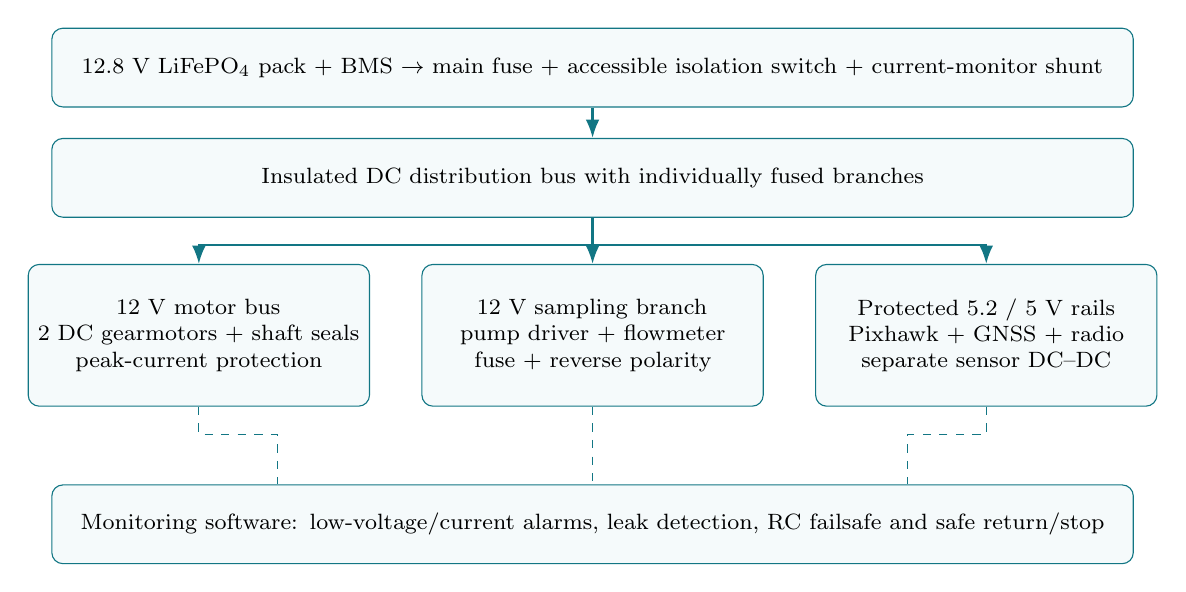
\begin{tikzpicture}[>=Latex,font=\footnotesize,
 bus/.style={draw=teal,rounded corners,fill=cream,text width=13.5cm,minimum height=10mm,align=center},
 branch/.style={draw=teal,rounded corners,fill=cream,text width=4.1cm,minimum height=18mm,align=center},
 arr/.style={-Latex,thick,teal}]
\node[bus] (battery) at (0,0) {12.8 V LiFePO$_4$ pack + BMS $\rightarrow$ main fuse + accessible isolation switch + current-monitor shunt};
\node[bus] (distribution) at (0,-1.4) {Insulated DC distribution bus with individually fused branches};
\node[branch] (motor) at (-5.0,-3.4) {12 V motor bus\\2 DC gearmotors + shaft seals\\peak-current protection};
\node[branch] (pump) at (0,-3.4) {12 V sampling branch\\pump driver + flowmeter\\fuse + reverse polarity};
\node[branch] (logic) at (5.0,-3.4) {Protected 5.2 / 5 V rails\\Pixhawk + GNSS + radio\\separate sensor DC--DC};
\node[bus] (safety) at (0,-5.8) {Monitoring software: low-voltage/current alarms, leak detection, RC failsafe and safe return/stop};
\draw[arr](battery)--(distribution);
\foreach \x in {motor,pump,logic} \draw[arr] (distribution.south) -- ++(0,-.35) -| (\x.north);
\draw[dashed,teal] (motor.south) -- ++(0,-.35) -| ([xshift=-4cm]safety.north);
\draw[dashed,teal] (pump.south) -- ++(0,-.35) -| (safety.north);
\draw[dashed,teal] (logic.south) -- ++(0,-.35) -| ([xshift=4cm]safety.north);
\end{tikzpicture}
\caption{Power-distribution concept with genuinely parallel fused motor, pump and logic branches. Dashed paths denote monitoring/fault signalling rather than physical series wiring.}\end{figure}
\textbf{Controller power:} The Holybro PM02 V3 \emph{analog} offers regulated 5.2 V up to 3 A from a 2S--12S input and is the appropriate signal class for Pixhawk 6C; the PM02D digital variant is explicitly \emph{incompatible} with Pixhawk 6C. The PM02 V3 is \emph{not} a high-current supply for servos, pump or motors \cite{PM02D}. Confirm cable/connector pinout and analog voltage/current scaling for the selected Pixhawk 6C; the separately listed PM02D digital variant must not be substituted. Use fused motor and pump circuits; fuses protect wires, not simply the device. \textbf{Battery charging:} A representative Bioenno 12 V 20 Ah LiFePO$_4$ pack includes a protection module with 30 A continuous discharge and specifies a suitable 14.6 V charger (manufacturer example 4 A) \cite{Bioenno}. Do not charge LiFePO$_4$ with an unmatched lead-acid or LiPo charger. Charge in a dry supervised location, disconnected from the boat loads, with supplier-approved charger and appropriate temperature constraints.

\begin{table}[H]\centering\footnotesize
\caption{Averaged survey-power allowances at the DC bus: \emph{engineering assumptions}, not manufacturer measurements.}
\begin{tabularx}{\linewidth}{@{}Yrr@{}}\toprule
Component / combined function & Track A W & Track B W\\\midrule
Two GM25 motors, \emph{assumed average} (combined) & 50 & 30\\
Autopilot, GNSS, RC receiver & 6 & 6\\
Telemetry / logging & 4 & 2\\
Camera/computer & 9 & 0\\
Pump, \emph{duty-averaged} & 12 & 6\\
Conversion/misc. margin & 7 & 4\\\midrule
\textbf{Estimated average} & \textbf{88} & \textbf{48}\\\bottomrule\end{tabularx}\end{table}
\[E_{\mathrm{nom}}=12.8\times20=256\,\mathrm{Wh},\qquad E_{\mathrm{usable}}=0.80\times256=204.8\,\mathrm{Wh},\qquad t=E_{\mathrm{usable}}/P_{\mathrm{average}}.\]
\begin{table}[H]\centering\footnotesize
\caption{Illustrative 12.8 V, 20 Ah battery operating time: energy-only estimates, ignoring rate/thermal limits and unmodelled loads. Source: \texttt{data/power\_endurance.csv}.}
\begin{tabularx}{\linewidth}{@{}Yrrrr@{}}\toprule
Scenario & Avg W & h & Energy for 2h & 2h energy gate\\\midrule
Track B economical & 48 & 4.27 & 96 Wh & Pass\\
Track A planned & 88 & 2.33 & 176 Wh & Pass (narrow)\\
Track A difficult water & 125 & 1.64 & 250 Wh & Fail\\
High-drive manoeuvres & 180 & 1.14 & 360 Wh & Fail\\
Two GM25 near stall + accessories, illustrative & 380 & 0.54 & 760 Wh & Fail; fuse/thermal hazard\\\bottomrule\end{tabularx}\end{table}
\textbf{Critical current warning:} The Cytron GM25 data give a $<16$ A \emph{stall} current per motor at 12 V. For two motors, this is a theoretical upper bound of $<32$ A before pump and avionics; blocked propellers can create a surge that defeats a modest 30 A BMS or overloads a branch. The normal 2.7 A rated per motor \emph{does not} define maximum draw. Fit independent branch fuses, overcurrent shutdown, sealed shafts, and qualify the motor-driver thermal behaviour. The 48 and 88 W survey budgets are \emph{illustrative allowances} and must be replaced with logged bus current, measured propeller-water load and pump duty cycle. 

\section{Time budget and survey choices}
Track A illustrative path: five $20$-m lanes plus four $5$-m lateral moves gives $120$ m. At an assumed $0.25$ m/s the ideal transit is $8$ min. A 60-min effective sensing period plus 25 min setup, turns, recovery, QC and map generation totals $93$ min. A $0.50$-L/min fully interrogated flow yields $30$ L in the sensing period, \emph{not} $30$ L per map cell. Sensor sampling time and intake-delay calibration matter.

Track B illustrative workflow: 16 stations, 1 L per site, effective pumping $1.5$ L/min, $1.2$ min/station for handling and $3$ min/station portable image processing; add 18 min survey movement/setup/mapping. The total is about $95.9$ min. Changing image time to 5 min/site raises it above 120 min. Field concentration and sampling statistics impose a stricter constraint: at around $3.12$ particles/L, a 1-L sample expects only 3.12 particles, equivalent to $57\%$ approximate Poisson standard error \emph{before} sensor losses. The first demonstration should specify a minimum reporting volume and show uncertain/insufficient-count cells rather than inventing a smooth precise heat map.

\section{Risk controls, procurement order and decision}
\begin{enumerate}[leftmargin=*]
\item \textbf{Float test first:} assemble sealed pontoons, weigh all components, add ballast to 22 and 30 kg, check reserve freeboard, trim and wave splash under stationary and moving load.
\item \textbf{Then drive/power test:} two approved-source geared DC motors with water-isolated shafts, propellers and matched DC drivers, current limit and speed tests at full mass. Inspect for overheating and waterproof cable glands.
\item \textbf{Autopilot and RC:} flash appropriate Rover firmware, configure boat class and motor layout, test manual/RTL/Loiter and safe response to link or GNSS loss while tethered.
\item \textbf{Sample circuit:} bench-test the selected pump's \emph{actual} flow through chosen strainers/filter and tubing at target depth; verify sampled volume and cleaning blanks.
\item \textbf{Timing and credibility:} time full 16-sample shoreline chain or Track A effective observed-volume throughput; reject any concept unable to create an auditable map within 120 min.
\item \textbf{Procurement and local radio:} request quotations from university-registered electronics/hardware suppliers, confirm Malaysia radio approval, battery transport/charging and replacement parts.
\end{enumerate}
\textbf{Revised V2.3 concept (procurement-compliant motor shortlist, marine performance unconfirmed):} two 0.9-m $\times$ 0.2-m sealed pontoons; two approved Cytron GM25 brushed geared motors \emph{mounted in a dry compartment} with independently qualified shafts/seals, guards and compatible Cytron two-channel brushed driver; Pixhawk 6C or a proven alternative controller subject to approved-supplier quotation; calibrated Cytron R385 sampling pump with volume/flow verification; and a correctly fused battery with measured discharge margin. A sealed-underwater propulsor remains a \textbf{registered-supplier RFQ or Shopee-variant qualification gap}; it is not legitimate to purchase directly from a maker that is not on the provided list. \emph{Do not claim a two-hour field-ready boat based on motor shaft-power alone.} The original approximately 22-kg wet mass is an illustrative allowance, not an as-built bill of materials.

\section{V2.3 procurement-ready basket and transparent cost gap}
The prices below are \emph{a purchase-planning example}, not a full field-boat quotation. This basket supports \textbf{bench calibration, low-power position logging and a short-duration manually controlled proof-of-concept}. The selection uses one reasonably priced component from each function; it deliberately does not claim that a short-test LiPo is capable of a 120-minute field mission.

\begin{table}[H]\centering\footnotesize
\caption{One-unit price-backed bench/prototype basket. Each hyperlink leads to the approved supplier's specific item listing. All values in RM (2 November 2026).}
\begin{tabularx}{\linewidth}{@{}Y r r r@{}}\toprule
Component (supplier hyperlink) & Qty & Unit RM & Line RM \\\midrule
\href{https://my.cytron.io/c-wireless-devices/c-wifi/p-nodemcu-esp32-with-expansion-board}{NodeMCU ESP32, Cytron} & 1 & 29.00 & 29.00\\
\href{https://my.cytron.io/c-other-wireless/p-lc76g-multi-gnss-module-supports-gps-bds-glonass-galileo-qzss}{LC76G multi-GNSS, Cytron} & 1 & 69.00 & 69.00\\
\href{https://my.cytron.io/c-sensor/c-others-sensor/p-gravity-analog-turbidity-sensor-for-arduino-41626}{SEN0189 turbidity, Cytron} & 1 & 55.00 & 55.00\\
\href{https://my.cytron.io/p-r385-dc12v-diaphragm-water-pump}{R385 pump, Cytron} & 1 & 10.90 & 10.90\\
\href{https://my.cytron.io/c-dc-geared-motor/p-12v-980rpm-2.3kgfcm-high-power-brushed-dc-geared-motor}{GM25-20K dry-test motors, Cytron} & 2 & 49.00 & 98.00\\
\href{https://my.cytron.io/c-motor-driver/c-dc-motor-driver/p-10amp-5v-30v-dc-motor-driver-2-channels}{MDD10A, Cytron} & 1 & 108.78 & 108.78\\
\href{https://my.cytron.io/p-g1-2-half-effect-water-flow-sensor-yf-s201}{YF-S201 flowmeter, Cytron} & 1 & 49.00 & 49.00\\
\href{https://www.gie.com.my/shop.php?action=wireless/wifi/esp32_cam}{ESP32-CAM, GI Electronic} & 1 & 37.00 & 37.00\\
\href{https://my.cytron.io/p-outdoor-ip65-water-proof-enclosure-with-abs-plate}{IP65 box (small variant), Cytron} & 1 & 35.00 & 35.00\\
\href{https://my.cytron.io/p-hotrc-6-channels-rc-radio-transmitter-and-receiver}{HotRC TX + RX, Cytron} & 1 & 109.00 & 109.00\\
\href{https://my.cytron.io/p-lipo-rechargeable-battery-11.1v-5200mah}{3S 5.2 Ah LiPo, Cytron} & 1 & 155.00 & 155.00\\
\href{https://my.cytron.io/p-multi-function-lipo-balance-charger-13853}{B6AC balance charger, Cytron} & 1 & 95.00 & 95.00\\\midrule
\textbf{Documented listed-price subtotal} & & & \textbf{850.68}\\
\bottomrule\end{tabularx}\end{table}
\textbf{Cost exclusions:} delivery/tax, water-safe hoses and fittings, filter and reference-counting consumables, buffer and calibration chemicals, reference microscopy, proper waterproof cable glands, sensor ADC if needed, fuse/wire/kill switch, motor/thruster mounts, buoyant hull and frame, battery protection, sensors for leak/current, waterproof electronics mounting, field-certified power supply and, above all, \textbf{2 marine-qualified propulsion units/shaft seals + their correctly matched controllers + Pixhawk 6C / power module}. The RM850.68 is \emph{not} a full floating survey system price, and the YF-S201 would not validate the 0.5 L/min flow assumption.

\subsection{Three staged purchase decisions}
\begin{enumerate}[leftmargin=*]
\item \textbf{Purchase now only after approval (low-risk):} turbidity module, R385, ESP32, GNSS, calibrated beaker/scale; use indoor tap-water and microplastic reference trials before installing the components on a boat.
\item \textbf{Quote before hull freeze (high-risk):} 2 registered-supplier or procurement-cleared Shopee thrusters/ESCs \emph{or} a fully specified waterproof alternative; Pixhawk/GNSS/compass assembly, RC interface, 12.8 V 20 Ah LiFePO$_4$ with current-appropriate BMS/charger; two sealed pontoons and waterproof fittings. Solicit through Cytron, Element14, RS, DigiKey, Autobotic, Mybotic, Vanguard and the registered hardware contacts; accept only an actual supplier response as a price.
\item \textbf{Defer until calibration evidence:} RM1,135 industrial optical turbidity probe, more expensive image acquisition, GPS accuracy upgrades and retained 16-L sample storage. These require proof that the measured variable predicts actual MP concentrations better than the cheaper prototype.
\end{enumerate}

\subsection{RFQ form and verification before raising a purchase order}
\begin{table}[H]\centering\footnotesize
\caption{Fields to request from registered suppliers; a missing quotation is a procurement blocker, not a zero-cost line item.}
\begin{tabularx}{\linewidth}{@{}L{3.6cm}Y@{}}\toprule
RFQ item & Required written evidence \\\midrule
Marine propulsion set & Exact part model, qty 2 thrust units + qty 2 reversible ESCs, voltage, continuous/start current, guards, cable glands and water rating, unit/total MYR, warranty and lead time\\
Navigation/RC & Pixhawk 6C revision, GNSS/compass and antenna options, PM02D or correct power module, complete RC receiver data interface and failsafe, availability and purchase total\\
Energy subsystem & 12.8 V 20 Ah LiFePO$_4$ pack, continuous/peak BMS rating, included cell protection, charger model, connector, weight, shipping limitations and total MYR\\
Hull + wetted parts & Watertight pontoon material, sealed displacements, frame/bulkhead fabrication, fittings, tubing, cleanable mesh, microplastic contamination controls and total MYR\\
\bottomrule\end{tabularx}\end{table}

\textbf{Order-release gate:} sign off the selected architecture, full all-up mass, two-hour energy feasibility, wet-sensor QC protocol, safe recovery and current limits \emph{before} spending on the expensive field package. Confirm any import freight and Malaysian radio compliance. Only if no registered supplier can fulfil should the team contact Procurement for a non-registered purchase exception.

\section{V2 measurement validity and field-test gates}
The uploaded project brief requires a \emph{two-dimensional MP concentration map with demonstrable links to true MP and an appropriate laboratory reference}. The talk supplied by the supervisors describes direct measurements and image-based approaches as open options, and specifically cautions that image methods require a calibration relationship. Accordingly:
\begin{enumerate}[leftmargin=*]
\item \textbf{Reference protocol:} obtain duplicate, known-volume samples across clean and contaminated water conditions, filter and microscopy-count, and document blanks and recovery. Record concentration as \(C_{\rm MP}=N_{\rm confirmed}/V_{\rm sampled}\), with the reporting size window and sample volume.
\item \textbf{Proxy protocol:} record contemporaneous turbidity/optical intensity and environmental confounders at the same sample locations and times. Test between-day and across-location generalisation instead of relying on a high in-sample correlation.
\item \textbf{Survey protocol:} log fix quality, latitude, longitude, timestamps, transect ID, stage of processing, flow/volume and uncertainties; map blank/insufficient-data cells explicitly instead of interpolating false precision.
\item \textbf{Time and payload:} preserve the V1 two-hour and \(20\times20\,\mathrm m\) target, but qualify any result as a measured count, calibrated estimate or \emph{uncalibrated turbidity proxy}; they are not interchangeable.
\end{enumerate}
\textbf{Critical V2 change relative to V1:} low-cost products are explicitly \emph{calibration and development candidates}, not automatic replacement for marine-rated navigation, propulsion, power or an MP-specific laboratory assay. All compared item prices are linked to an approved supplier, and the three high-value unresolved packages remain labelled RFQ.

\printbibliography[title={References and manufacturer documentation}]
\end{document}